\documentclass[11pt]{article}
%%% style file you will need for some commands%%%%%%%%%%%%%%%%%%%%%%
%% aahomework is the style file I have used to typeset many commands, feel free to use them in your solutions.
%% bear in mind that if you need to define your command then you will have to make sure that it is not in conflict to my pre-defined command. Otherwise you will need to either use
%% commands defined by me or edit the style file appropriately.
\usepackage[dvipsnames]{xcolor}
\usepackage{aahomework}
\usepackage{tikz}
\usepackage{tipa}
\usepackage{color}
\usepackage{tcolorbox}
\usepackage{graphicx}
\graphicspath{ {images/} }

\newcommand*\circled[1]{\tikz[baseline=(char.base)]{
            \node[shape=circle,draw,inner sep=2pt] (char) {#1};}}
%%%the \circled command has been used to create text inside circle for grading table.

%%%\geometry{letterpaper, textwidth=17cm, textheight=22cm}

%%%%%%%%%%%%%%%%%%%%%%%%%%%%%%%%%%%% the following is for the cover sheet--FILL IN appropriately%%
\newcommand{\mycourse}{Introduction to Computer Linguistics 8.1008}
\newcommand{\semesteryear}{Spring 2016}
\newcommand{\myname}{Timothy Fairman, Kaitlin Hipkin, Tyler Wilgenbusch}  %%<<<<<<<<<<<<<<<|========================================= (please put your name here)==========
\newcommand{\hwnumber}{2} %%<<<<<<<<<<<<<<<|========================================= (please put HW number here, e.g. 1,2,3...)==========

%%%%%%%%%%%%%%%%%%%%%%%%%%%%%%%%%%%%%% following is NOT to be edited, DO NOT type anything here, it will receive inputs from what you fill above%%%%%%%%%%%%%%%%%%
\title{Homework \hwnumber} %% DO NOT type in HW number here
\author{\myname} %% DO NOT type in your name here.
\date{\textbf{\mycourse} \hfill {\today} \hfill \textbf{\semesteryear}} %% DO NOT TYPE in mycourse and/or quarteryear values
%%%%%%%%%%%%%%%%%%%%%%%%%%%%%%%%%%%%%%%%%%%%%%%%%%%%%%%%%%%%%%%%%%%%%%%%%%%%%%%%%%%%%%%%%%%%%%%%%%%%%%%%%%%%%%%%%%%%%%%%%%%%%%%%

\setlength{\parindent}{0pt} %% paragraphs will not be indented
\setlength{\parskip}{.25cm} %% space between paragraphs
\linespread{1.1}

\begin{document}
\thispagestyle{empty} %%this is to supress the page number on the cover page

\clearpage %% these are to reset the page number for the first page of your homework to 1.
\pagenumbering{arabic} %% these are to reset the page number for the first page of your homework to 1.
\maketitle

%%%%%%%%%%%%%%%%%%%%%%%%%%%%%%%%% you may start typing below%%%%%%%%%%%%%%%%%%%%%%%%%%%%%%%%%%%%%%%
%% In my style file aahomework.sty I have defined two environments "problem" and "solution" that can be used to type in your question and answer respectively as shown below.%%

\begin{problem}{1}
\textbf{Morphological Parsing}

Give a morphological analysis of the following words,
\begin{tcolorbox}
	\textbf{English}: printer, underdetermination, incremental \\
	\textbf{German}: Versprecher, Ansprechpartner, {\"u}bergezogener
\end{tcolorbox}

The morphological analysis should be broken down as follows:
\begin{itemize}
	\item Say of each simplex morpheme whether it is a stem, a base, a root, a prefix, a derivational, or an inflectional suffix.
	\item Give the order of composition, indicating at each level which morpheme is the base.
	\item Mark each base for its POS.

\end{itemize}


Example: \textbf{unabsehbar}
\begin{itemize}
	\item Verbal Root (=base): \textbf{seh-} combines with derivational prefix \textbf{ab-} to yield complex \textit{verbal base} \textbf{abseh-}

	\item Verbal Base: \textbf{abseh-} combines with derivational suffix \textbf{-bar} to yield adjective (or \textit{adjectival base}) \textbf{absehbar}

	\item Adjectival Base: \textbf{absehbar} combines with prefix \textbf{un-} to yield \textit{adjective} \textbf{unabsehbar}. 
\end{itemize}

\end{problem}

\newpage

\begin{solution}
The definitions for the various symbols for the \textit{subscripts} are as follows:
\begin{itemize}
	\item $N$ : Noun
	\item $V$ : Verb
	\item $Adj.$ : Adjective
	\item $root$ : The root of a word; i.e. the minimal free morpheme of the word
	\item $base$ : A base of the word; i.e. a possibly complex free morpheme of the word
	\item $stem$ : A stem of the word; i.e. an \textit{inflected form} of another base
	\item $der. suf.$ : A derivational suffix of a word/base/stem
	\item $der. pre.$ : A derivational prefix of a word/base/stem
	\item $inf. suf.$ : An inflectional suffix of a word/base/stem
	\item $inf. pre.$ : An inflectional prefix of a word/base/stem
	\item $inf. cir.$ : An inflectional circumfix of a word/base/stem
\end{itemize}

\textbf{English}:
\begin{enumerate}
	\item \textbf{printer}
		\begin{itemize}
			\item \textbf{print}$_{(V|root, base)}$ + \textbf{-er}$_{(der. suf.)}$ yields \textbf{printer}$_{(N)}$
		\end{itemize}
	\item \textbf{underdetermination}
		\begin{itemize}
			\item \textbf{determin}(e)$_{(V|root, base)}$ + \textbf{-ate}$_{(der. suf.)}$ yields \textbf{determina}(te)$_{(Adj.|base)}$
			\item \textbf{determina}(te)$_{(Adj.| base)}$ + \textbf{-tion}$_{(der. suf.)}$ yields \textbf{determination}$_{(N|base,stem)}$
			\item \textbf{under-}$_{(inf. pre.)}$ + \textbf{determination}$_{(N| base,stem)}$  yields \textbf{underdetermination}$_{(N)}$
		\end{itemize}
	\item \textbf{incremental}
		\begin{itemize}
			\item \textbf{incre}(ase)$_{(V|root, base)}$ + \textbf{-ment}$_{(der. suf.)}$ yields \textbf{increment}$_{(N|base)}$
			\item \textbf{increment}$_{(N|base)}$ + \textbf{-al}$_{(der. suf.)}$ yields \textbf{incremental}$_{(Adj)}$
		\end{itemize}
\end{enumerate}

\newpage

\textbf{German}:
\begin{enumerate}
	\item \textbf{Versprecher}
		\begin{itemize}
			\item \textbf{sprech}(en)$_{(V|root, base)}$ + \textbf{-er}$_{(der. suf.)}$ yields \textbf{Sprecher}$_{(N|base, stem)}$
			\item \textbf{Ver-}$_{(inf. pre.)}$ + \textbf{Sprecher}$_{(N|base, stem)}$ yields \textbf{Versprecher}$_{(N)}$
		\end{itemize}
	\item \textbf{Ansprechpartner}: A \textit{compound word} compose of two words: \textbf{ansprech}(en) and \textbf{Partner}
		\begin{enumerate}
			\item \textbf{ansprech}(en)
				\begin{itemize}
					\item \textbf{an-}$_{(inf. pre.)}$ + \textbf{sprech}(en)$_{(V|root, base, stem)}$  yields \textbf{ansprech}(en)$_{(V|base)}$
				\end{itemize}
			\item \textbf{Partner}
				\begin{itemize}
					\item \textbf{part}$_{(V|root, base)}$ + \textbf{-ner}$_{(der. suf.)}$ yields \textbf{Partner}$_{(N|base, stem)}$
				\end{itemize}
			The \textit{verbal base} \textbf{ansprech}(en) combines with the \textit{noun base} \textbf{Partner} to yield the \textit{noun} \textbf{Ansprechpartner}
		\end{enumerate}
	\item \textbf{{\"u}bergezogener}
		\begin{itemize}
			\item \textbf{ge-}$_{(inf. cir.)}$ + \textbf{zieh}(en)$_{(V|root, base, stem)}$ + \textbf{-en}$_{(inf. cir.)}$ yields \textbf{gezogen}$_{(V|base, stem)}$
			\item \textbf{{\"u}ber-}$_{(inf. pre.)}$ + \textbf{gezogen}$_{(V|base)}$  yields \textbf{{\"u}bergezogen}$_{(V|base)}$
			\item \textbf{{\"u}bergezogen}$_{(V|base)}$ + \textbf{-er}$_{(der. suf.)}$ yields \textbf{{\"u}bergezogener}$_{(Adj.)}$
		\end{itemize}
\end{enumerate}
\end{solution}

\vspace*{0.5cm} %% this is to put some vertical space betwen the next problem and the previous solution. You can change the value to something more appropriate.

\begin{problem}{2}
\textbf{Plurals}

Is the English plural formation really completely regular? List the allomorphs of the regular English plural morpheme and give three plural forms that are not formed regularly.
\end{problem}

\begin{solution}
The English morpheme for regular plurals ($<$+Pl$>$) is realised by 3 different allomorphs:
\begin{center}
$[$\textipa{z}$]$ : dog\textcolor{red}{s}; $[$\textipa{s}$]$ : cat\textcolor{red}{s}; $[$\textipa{iz}$]$ : fox\textcolor{red}{es}
\end{center}
Three words that have irregular plural forms are: \underline{mice} (plural of mouse), \underline{geese} (plural of goose), and \underline{die} (plural of dice). 

\end{solution}

\vspace*{0.5cm}

\begin{problem}{3}
\textbf{Words}

Give short definitions (at most 2 lines of text each) for the following terms:
\begin{itemize}
	\item Word form
	\item Grammatical word
	\item Lexeme
\end{itemize}

\end{problem}

\begin{solution}
\begin{itemize}
	\item Word form - A sequence of phonemes or graphemes that one particular lexeme can take.  For example, the lexeme TALK can have the word forms \textbf{talk} and \textbf{talks}.
	\item Grammatical word - A pair of phonemes or graphemes and a grammatical classification (i.e. how that word can be used in a sentence grammatically).
	\item Lexeme - The root element of a word which is stored in the mental lexicon.  This is the part of the word that we attach \textit{meaning} to.
\end{itemize}
\end{solution}

\vspace*{0.5cm}

\begin{problem}{4}
\textbf{Productivity}

Describe briefly the relation between productivity, rule, and blocking in morphology (at most
5 lines of text).

\end{problem}

\begin{solution} \\
In terms of morphology, \textit{productivity} is process that can be applied to arbitrary new words that appear in a language; i.e. the conjugation \textit{inflection} of regular of new verbs that appear in a language.  A \textit{rule} is used when creating new lexemes or words with a different meanings.  Rules are typically seen when adding suffixes or prefixes to existing words to create new ones with different meanings. \textit{Blocking} is simply the ``blocking'' of a regular word form by an irregular one; i.e. using the irregular plural ``mice'' instead of ``mouses''.
\end{solution}

\vspace*{0.5cm}
\newpage

\begin{problem}{5}
\textbf{Forms of Derivation}

Give 2 German and 2 English examples each for the following types of derivation:
\begin{itemize}
	\item Compounding
	\item Conversion
	\item Clipping
\end{itemize}

Do \textbf{not} use examples from the lecture slides.

\end{problem}

\begin{solution}
\begin{itemize}
	\item Compounding : occurs when two free morphemes are put together to form one word.
	\begin{itemize}
		\item English : \textbf{bittersweet}, \textbf{smalltalk} 
		\item German : \textbf{Schlafzimmer}, \textbf{Spielplatz}
	\end{itemize}
	\item Conversion : occurs when a word changes syntactic category, with a possible stem change.
	\begin{itemize}
		\item English : salt(Noun) $\rightarrow$ \textbf{salty}(Adjective), fun(Noun) $\rightarrow$ \textbf{funny}(Adjective)
		\item German : lesen(Verb) $\rightarrow$ \textbf{Leser}(Noun), fahren(Verb) $\rightarrow$ \textbf{Fahrer}(Noun)
	\end{itemize}
	\item Clipping : occurs when a word is shortened and the new word becomes part of the lexicon.
	\begin{itemize}
		\item English : \textbf{exam}(ination), \textbf{lab}(oratory)
		\item German : \textbf{Pils}(ner), \textbf{U}(ntersee)\textbf{-boat}
	\end{itemize}
\end{itemize}
\end{solution}

\vspace*{0.5cm}
\newpage

\begin{problem}{6}
\textbf{X-language Verbal Morphology}

X-language is a variant of a language spoken somewhere in Africa. As the following example shows, X-language's verbs are so complex that they can sometimes convey the meaning of an entire sentence on their own.

\begin{tabular}{l l | l l} 
\hline atalopenda & ``he will like me'' & atalopiga & ``he will beat me'' \\
atakupenda & ``he will like you'' & atakupiga & ``he will beat you'' \\
atampenda & ``he will like him'' & atampiga & ``he will beat him'' \\
atanipenda & ``he will like us'' & analopiga & ``he is beating me'' \\
atawapenda & ``he will like them'' & anakupiga & ``he is beating you'' \\
lotakupenda & ``I will like you'' & anampiga & ``he is beating him'' \\
lotampenda & ``I will like him'' & amekupiga & ``he has beaten you'' \\
lotawapenda & ``I will like them'' & amelopiga & ``he has beaten me'' \\
utalopenda & ``you will like me'' & amempiga & ``he has beaten him'' \\
utampenda & ``you will like him'' & alilopiga & ``he beat me'' \\
nitampenda & ``we will like him'' & alikupiga & ``he beat you'' \\
watampenda & ``they will like him'' & alimpiga & ``he beat him'' \\
atakusumbau & ``he will annoy you'' & wamenilipa & ``they have paid us'' \\
unamsumbau & ``you are annoying him'' & nilikulipa & ``we paid you'' \\ \hline
\end{tabular}

\begin{description}
	\item[a.] Give the X-language morphemes corresponding to the following English morphemes: \textit{I}, \textit{me}, \textit{us}, \textit{you} (as subject), \textit{you} (as object), \textit{he}, \textit{him}, \textit{they}, \textit{them}, \textit{-ed} (past tense), \textit{will} (future), \textit{is+ -ing} (present progressive), \textit{has+ -en} (present perfect), and the verbal roots \textit{like}, \textit{annoy}, \textit{beat}, and \textit{pay}.
	\item[b.] Illustrate how the morphemes combine by giving all inflected forms of the X-language equivalent of the verb \textbf{annoy} for past and future in the $1^{st}$, $2^{nd}$, and $3^{rd}$ person singular and plural subject and $2^{nd}$ person object, with their translation into English.
\end{description}

\end{problem}

\newpage

\begin{solution}

\begin{description}
\item[a.] The X-language ``sentence'' structure is broken up into 4 major, distinct parts: \\
\textcolor{red}{Subject} - \textcolor{OliveGreen}{Tense} - \textcolor{blue}{Object} - \textcolor{BurntOrange}{Verb Root} \\
The X-language morphemes are mapped to the English morphemes as follows:

\begin{tabular}{l l | l l | l l}
English Pronoun & X-language & English Tense & X-language & English Verb & X-language \\ \hline 
I & ``\textcolor{red}{lo}'' & Past (-ed) & ``\textcolor{OliveGreen}{li}'' & like & ``\textcolor{BurntOrange}{penda}'' \\
me & ``\textcolor{blue}{lo}'' & Future (will) & ``\textcolor{OliveGreen}{ta}'' & annoy & ``\textcolor{BurntOrange}{sumbau}'' \\
we & ``\textcolor{red}{ni}'' & Present Pro. & ``\textcolor{OliveGreen}{na}'' & beat & ``\textcolor{BurntOrange}{piga}'' \\
us & ``\textcolor{blue}{ni}'' & Present Per. & ``\textcolor{OliveGreen}{me}'' & pay & ``\textcolor{BurntOrange}{lipa}'' \\
you (Sub.) & ``\textcolor{red}{u}'' & & & &  \\
you (Obj.) & ``\textcolor{blue}{ku}'' & & & & \\
he & ``\textcolor{red}{a}'' & & & & \\
him & ``\textcolor{blue}{m}'' & & & & \\
they & ``\textcolor{red}{wa}'' & & & & \\
them & ``\textcolor{blue}{wa}'' & & & & \\
\end{tabular}

\textbf{NOTE}: The plural forms of ``you'' ($2^{nd}$ person subject/object) are the same as the singular forms in both the X-language and English.

\item[b.] The following two tables both use the $2^{nd}$ person object (you/``\textcolor{blue}{ku}'') in their translations.

Inflection tables for ANNOY (``\textcolor{BurntOrange}{sumbua}''):

\begin{tabular}{l l | l l}
Case & Subject & Past Tense(``\textcolor{OliveGreen}{li}'') & Translation \\ \hline
$1^{st}$ Person Singular & I/``\textcolor{red}{lo}'' & \textcolor{red}{lo}\textcolor{OliveGreen}{li}\textcolor{blue}{ku}\textcolor{BurntOrange}{sumbau} & I annoyed you \\
$1^{st}$ Person Plural & we/``\textcolor{red}{ni}'' & \textcolor{red}{ni}\textcolor{OliveGreen}{li}\textcolor{blue}{ku}\textcolor{BurntOrange}{sumbau} & we annoyed you \\
$2^{nd}$ Person Singular & you/``\textcolor{red}{u}'' & \textcolor{red}{u}\textcolor{OliveGreen}{li}\textcolor{blue}{ku}\textcolor{BurntOrange}{sumbau} & you annoyed you \\
$2^{nd}$ Person Plural & you/``\textcolor{red}{u}'' & \textcolor{red}{u}\textcolor{OliveGreen}{li}\textcolor{blue}{ku}\textcolor{BurntOrange}{sumbau} & you annoyed you \\
$3^{rd}$ Person Singular & he/``\textcolor{red}{a}'' & \textcolor{red}{a}\textcolor{OliveGreen}{li}\textcolor{blue}{ku}\textcolor{BurntOrange}{sumbau} & he annoyed you  \\
$3^{rd}$ Person Plural & they/``\textcolor{red}{wa}'' & \textcolor{red}{wa}\textcolor{OliveGreen}{li}\textcolor{blue}{ku}\textcolor{BurntOrange}{sumbau} & they annoyed you \\ \hline
\end{tabular}

\begin{tabular}{l l | l l}
 
Case & Subject & Future Tense(``\textcolor{OliveGreen}{ta}'') & Translation \\
$1^{st}$ Person Singular & I/``\textcolor{red}{lo}'' & \textcolor{red}{lo}\textcolor{OliveGreen}{ta}\textcolor{blue}{ku}\textcolor{BurntOrange}{sumbau} & I will annoy you \\
$1^{st}$ Person Plural & we/``\textcolor{red}{ni}'' & \textcolor{red}{ni}\textcolor{OliveGreen}{ta}\textcolor{blue}{ku}\textcolor{BurntOrange}{sumbau} & we will annoy you \\
$2^{nd}$ Person Singular & you/``\textcolor{red}{u}'' & \textcolor{red}{u}\textcolor{OliveGreen}{ta}\textcolor{blue}{ku}\textcolor{BurntOrange}{sumbau} & you will annoy you \\
$2^{nd}$ Person Plural & you/``\textcolor{red}{u}'' & \textcolor{red}{u}\textcolor{OliveGreen}{ta}\textcolor{blue}{ku}\textcolor{BurntOrange}{sumbau} & you will annoy you \\
$3^{rd}$ Person Singular & he/``\textcolor{red}{a}'' & \textcolor{red}{a}\textcolor{OliveGreen}{ta}\textcolor{blue}{ku}\textcolor{BurntOrange}{sumbau} & he will annoy you  \\
$3^{rd}$ Person Plural & they/``\textcolor{red}{wa}'' & \textcolor{red}{wa}\textcolor{OliveGreen}{ta}\textcolor{blue}{ku}\textcolor{BurntOrange}{sumbau} & they will annoy you \\ \hline
\end{tabular}

\end{description}

\end{solution}

\vspace*{0.5cm}

\begin{problem}{7}
\textbf{Two-level Morphology for Regular English Past Tense.}

Suppose the grammatical form for the past tense of the English verb \underline{gaze} is $<$gaze,+V,+Past$>$ and for the verb \underline{walk} $<$walk,+V,+Past$>$, etc. while the surface forms are \textit{gazed} and \textit{walked}.

\begin{description}
	\item[a.] What would be the \textbf{underlying form} (showing morpheme and word boundaries) for these two past tense forms?
	
	\item[b.] What could an \textbf{FST for the lexical mapping} look like, i.e., an FST that transforms the grammatical form into the underlying form for all regular English verbs? Give the FST in the form of a graph, as in the lecture slides for the plural English FST.
	
	\item[c.] What could an \textbf{FST for the surface mapping} look like, i.e., an FST that transforms the underlying form into the surface form for all regular English verbs? Give the FST in the form of a graph, as in the lecture slides for the plural English FST.
\end{description}

Hint: The regular English past tense is formed by adding –ed to the base, unless the base ends in e; in the latter case only –d is added.

\end{problem}

\begin{solution}
\begin{description}
	\item[a.] The \textbf{underlying forms} of these two words after going through lexical mapping would be:
		\begin{itemize}
			\item \underline{gaze} $\rightarrow$ \textbf{gaze$\wedge$d\#}
			\item \underline{walk} $\rightarrow$ \textbf{walk$\wedge$d\#}
		\end{itemize}
		Where ``$\wedge$'' is the \textit{morpheme boundary} and ``\#'' is the \textit{word boundary}.

	\item[b.] The \textbf{FST for lexical mapping} for English regular past tense can be defined with the 7-tuple:
	Let $F = <Q, \Sigma, \Delta, q_{0}, F, \delta(q, w), \sigma(q, w)>$, such that:

	\begin{tabular}{l | l}
		$Q$ & $\{ q_{0}, q_{1}, q_{2}\}$ \\
		$\Sigma$ & $\{a, \ldots, z, +V, +Past\}$ \\
		$\Delta$ & $\{a, \ldots, z, \wedge, \# \}$ \\
		$q_{0}$ & $q_{0}$ \\
		$F$ & $\{ q_{2} \}$ \\
		$\delta(q, w)$ &  $\{ (q_{0},\{a, \ldots, z\},q_{0}), (q_{0}, +V, q_{1}), (q_{1}, +Past, q_{2}) \}$ \\
		$\sigma(q, w)$ & $\{ (q_{0},\{a, \ldots, z\},\{a, \ldots, z\}), (q_{0}, +V, \varepsilon), (q_{1}, +Past, \wedge d\#) \}$
	\end{tabular}

	\begin{figure}[h]
		\centering
		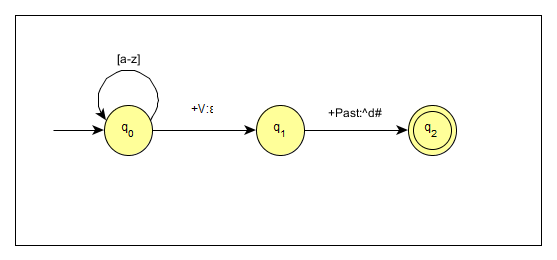
\includegraphics[width=10cm, height=5cm]{problem07partb} \\
		\caption{Lexical Mapping FST for English Past Tense}
	\end{figure}

	\item[c.] The \textbf{FST for surface mapping} for English regular past tense can be defined with the 7-tuple:
	Let $F = <Q, \Sigma, \Delta, q_{0}, F, \delta(q, w), \sigma(q, w)>$, such that:

	\begin{tabular}{l | l}
		$Q$ & $\{ q_{0}, q_{1}, q_{2}, q_{3}, q_{4}\}$ \\
		$\Sigma$ & $\{a, \ldots, z, \wedge, \# \}$ \\
		$\Delta$ & $\{a, \ldots, z\}$ \\
		$q_{0}$ & $q_{0}$ \\
		$F$ & $\{ q_{4} \}$ \\
		$\delta(q, w)$ &  $\{(q_{0},e,q_{0}), (q_{0}, \{a, \ldots\, z\} \cap \{e\}, q_{1}), (q_{0},\wedge, q_{2}), $ \\
		 &  $(q_{1},\{a, \ldots, z\} \cup \{\#\},q_{0}), (q_{1}, \wedge , q_{2}), (q_{2}, d, q_{3}), (q_{3}, \#, q_{4})\}$\\
		 & \\
		$\sigma(q, w)$ & $\{(q_{0},e,e), (q_{0}, \{a, \ldots\, z\} \cap \{e\},\{a, \ldots\, z\} \cap \{e\}), (q_{0},\wedge, \varepsilon), $ \\
		 &  $(q_{1},\{a, \ldots, z\} \cup \{\#\},\{a, \ldots, z\} \cup \{\#\}), (q_{1}, \wedge , e), (q_{2}, d, d), (q_{3}, \#, \varepsilon)\}$\\
	\end{tabular}

	\begin{figure}[h]
		\centering
		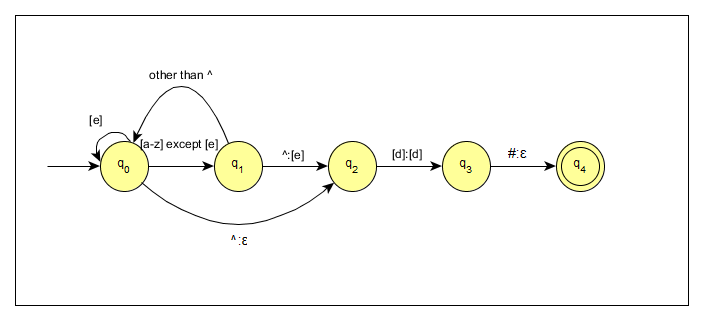
\includegraphics[width=13cm, height=6cm]{problem07partc} \\
		\caption{Surface Mapping FST for English Past Tense}
	\end{figure}

\end{description}

\end{solution}

\end{document}